\documentclass[preprint,12pt,aps,pra,showkeys,amsmath,amssymb,superscriptaddress,floatfix]{revtex4-2}
\usepackage[T1]{fontenc}
\usepackage[utf8]{inputenc}
\usepackage{amsmath,amssymb,amsthm,mathtools,mathrsfs}
\usepackage{microtype,booktabs,enumitem}
\usepackage{xcolor,tikz,etoolbox}
\usepackage[skins,breakable]{tcolorbox}
\usepackage{needspace}
% Keep diagram geometry independent of REVTeX preprint body spacing.
\AtBeginEnvironment{tikzpicture}{\linespread{1}\selectfont}
\usetikzlibrary{arrows.meta,positioning,calc,fit,decorations.pathreplacing}
\usepackage{graphicx}
\usepackage{hyperref}

\definecolor{MMBlue}{RGB}{0,82,155}
\definecolor{MMOrange}{RGB}{200,80,0}
\tikzset{
 mmnode/.style={draw=MMBlue,rounded corners=2pt,fill=MMBlue!4,align=left,execute at begin node={\raggedright},text width=5cm,font=\fontsize{10}{12}\selectfont,inner sep=6pt},
 mmimport/.style={mmnode,draw=black!65,fill=black!4},
 mmcandidate/.style={mmnode,draw=MMOrange,dashed,fill=MMOrange!5},
 mmrejected/.style={mmnode,draw=black,densely dotted,fill=black!8},
 mmproof/.style={->,thick,MMBlue},
 mmflow/.style={->,semithick,black!70},
 mmrepair/.style={->,dashed,thick,MMOrange},
 mmcandidatearrow/.style={->,dashed,semithick,MMOrange},
 mmnote/.style={font=\scriptsize,fill=white,inner sep=2pt,align=center}}

\usepackage[section]{placeins}
\setlength{\emergencystretch}{3em}
\setlist{itemsep=3pt,topsep=4pt}
\newtheorem{theorem}{Theorem}[section]
\newtheorem{proposition}[theorem]{Proposition}
\newtheorem{lemma}[theorem]{Lemma}
\newtheorem{corollary}[theorem]{Corollary}
\theoremstyle{definition}
\newtheorem{definition}[theorem]{Definition}
\newtheorem{example}[theorem]{Example}
\theoremstyle{remark}
\newtheorem{remark}[theorem]{Remark}
% Avoid isolated statement headings and single-line paragraph fragments.
\BeforeBeginEnvironment{theorem}{\Needspace{6\baselineskip}}
\BeforeBeginEnvironment{definition}{\Needspace{5\baselineskip}}
\BeforeBeginEnvironment{proposition}{\Needspace{5\baselineskip}}
\BeforeBeginEnvironment{lemma}{\Needspace{5\baselineskip}}
\BeforeBeginEnvironment{corollary}{\Needspace{5\baselineskip}}
\clubpenalty=5000
\widowpenalty=5000
\newcommand{\R}{\mathbb R}\newcommand{\Z}{\mathbb Z}\newcommand{\N}{\mathbb N}
\newcommand{\Pa}{\operatorname{Pa}}\newcommand{\Desc}{\operatorname{Desc}}
\newcommand{\cl}{\operatorname{cl}}\newcommand{\cost}{\operatorname{cost}}
\newcommand{\status}{\operatorname{status}}
% Faculty cards: a visual rail groups the five faculties within one agent.
% The rail has no arrowhead and does not represent a proof dependency.
\newcommand{\mmfacultybadge}[1]{%
 \node[circle,draw=MMBlue,line width=1pt,fill=white,
 minimum size=7mm,inner sep=0pt,font=\sffamily\small\bfseries,text=MMBlue]
 at ([xshift=15pt,yshift=-15pt]frame.north west) {#1};}
\newcommand{\mmfacultyrail}{%
 \draw[MMBlue!80,line width=1pt]
 ([xshift=15pt,yshift=2pt]frame.north west)--
 ([xshift=15pt,yshift=-2pt]frame.south west);}
\newtcolorbox{mmfacultybox}[2]{enhanced,breakable,
 colback=MMBlue!4,colframe=MMBlue!4,boxrule=0pt,arc=3pt,
 left=39pt,right=9pt,top=4pt,bottom=4pt,
 before skip=2pt,after skip=2pt,
 fontupper=\small\linespread{1.1}\selectfont,
 overlay unbroken={\mmfacultyrail\mmfacultybadge{#1}},
 overlay first={\mmfacultyrail\mmfacultybadge{#1}},
 overlay middle={\mmfacultyrail},overlay last={\mmfacultyrail}}
\newcommand{\mmfaculty}[3]{%
 \begin{mmfacultybox}{#1}{#2}
 {\sffamily\bfseries\color{MMBlue}#2}\par\smallskip #3
 \end{mmfacultybox}}
\newcommand{\agent}[9]{%
 \Needspace{8\baselineskip}
 \subsubsection{#1}
 \noindent\textbf{Object.} #2\par
 \noindent\textbf{Role.} #3\par\smallskip
 \mmfaculty{E}{Ego}{#4}
 \mmfaculty{M}{Memory}{#5}
 \mmfaculty{I}{Intellect}{#6}
 \mmfaculty{S}{Sense}{#7}
 \mmfaculty{A}{Action}{#8}
 \smallskip\noindent #9\par}

\usepackage{longtable,array,calc}
\providecommand{\tightlist}{\setlength{\itemsep}{2pt}\setlength{\parskip}{0pt}}
\makeatletter
\def\frontmatter@abstract@produce{\par\addvspace{\frontmatter@preabstractspace}%
\begingroup\prep@absbox\unvbox\absbox\post@absbox\endgroup
\addvspace{\frontmatter@postabstractspace}}
\makeatother
\newcommand{\field}[2]{\par\smallskip\noindent\textbf{#1.} #2\par}
\setlength{\emergencystretch}{5em}
\AtBeginEnvironment{verbatim}{\small\linespread{1.0}\selectfont}


\hypersetup{colorlinks=true,linkcolor=MMBlue,urlcolor=MMBlue,pdfauthor={Dibakar Sigdel}}

\begin{document}

\title{Optional Stopping for Bounded Stopping Times\\[4pt]\large An End-to-End Meta-Math Walkthrough}

\author{Dibakar Sigdel}

\affiliation{Mindverse Computing LLC, Lynnwood, WA 98087, USA}

\date{October 2026}

\begin{abstract}

Stopping retains exactly those increments whose inclusion was decided
before the next increment was observed. That predictability preserves
their zero conditional means. The report presents the target theorem,
declared imports, a dependency graph, five-faculty node contracts, a
continuous proof, a worked example, and a hypothesis-repair audit. It is
an authored mathematical exposition, not a deployed-agent transcript or
a formal proof-assistant certificate.

\end{abstract}\maketitle\linespread{1.12}\selectfont

\noindent\textbf{PS-03 / Probability and Stochastic Processes / Report v1}

\section{Target and import contract}

\begin{theorem}

Let \((M_n,\mathcal F_n)_{n\ge0}\) be an integrable real martingale:
\(M_n\) is \(\mathcal F_n\)-measurable, \(\mathbb E|M_n|<\infty\), and
\(\mathbb E[M_n\mid\mathcal F_{n-1}]=M_{n-1}\). Let \(\tau\) be a
stopping time with integer values and \(0\le\tau\le N\) almost surely
for some deterministic finite \(N\). Prove
\(\mathbb EM_\tau=\mathbb EM_0\). Also prove \((M_{n\wedge\tau})\) is a
martingale.

\end{theorem}

\subsection{Foundations and permitted imports}

Use linearity and the tower property of conditional expectation, and the
pull-out property for bounded measurable factors. A stopping time means
\(\{\tau\le n\}\in\mathcal F_n\). Finite sums of integrable variables
are integrable. The boundedness condition is on the time, not on sample
values of the martingale.

\clearpage\section{Node interaction workflow}

\begin{center}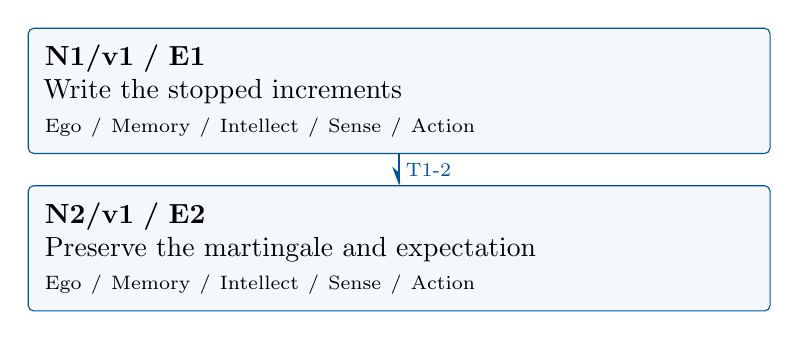
\begin{tikzpicture}[>=Stealth,x=1cm,y=1cm]

\node[mmnode,text width=9cm,minimum height=1.25cm] (N1) at (0,0.0) {\textbf{N1/v1 / E1}\\Write the stopped increments\\{\scriptsize Ego / Memory / Intellect / Sense / Action}};

\node[mmnode,text width=9cm,minimum height=1.25cm] (N2) at (0,-2.0) {\textbf{N2/v1 / E2}\\Preserve the martingale and expectation\\{\scriptsize Ego / Memory / Intellect / Sense / Action}};

\draw[mmproof] (N1.south) -- node[mmnote,right] {T1-2} (N2.north);

\end{tikzpicture}\end{center}

Each box is one mathematical agent containing all five faculties. Blue
arrows carry the versioned exports listed below. The layout gives a
reading order; only drawn arrows assert dependencies. Diagnostic repair
is separate from the proof DAG.

\subsection{Versioned evidence-transfer ledger}

\begingroup\small\linespread{1.05}\selectfont

\Needspace{5\baselineskip}\field{T1-2: N1/E1/v1 to N2}{\(M_{n\wedge\tau}=M_0+\sum_{k=1}^nD_k1_{\{\tau\ge k\}}\), with each
stopped increment conditionally mean zero.}

\field{Receiving activity}{N2.1}

\field{Compatibility}{E1/v1 and the deterministic bound \(\tau\le N\). Check: No limit of
expectations at an unbounded time is taken; the final stopped variable
equals \(M_{N\wedge\tau}\).}

\endgroup

\clearpage\section{Agent roles and five-faculty activities}\begingroup\small\linespread{1.05}\selectfont\setlist{itemsep=1pt,topsep=2pt}

\subsection{N1/v1: Write the stopped increments}

\field{Object and role}{Telescope the stopped path with indicators known at the preceding time.
\textbf{Local obligation:}
\(M_{n\wedge\tau}=M_0+\sum_{k=1}^nD_k1_{\{\tau\ge k\}}\), with each
stopped increment conditionally mean zero.}

\field{Inputs}{\(D_k=M_k-M_{k-1}\) and stopping time \(\tau\le N\).}

\mmfaculty{E}{Ego}{Publish E1/v1 only after establishing this obligation:
\(M_{n\wedge\tau}=M_0+\sum_{k=1}^nD_k1_{\{\tau\ge k\}}\), with each
stopped increment conditionally mean zero.}

\mmfaculty{M}{Memory}{\(D_k=M_k-M_{k-1}\) and stopping time \(\tau\le N\). Retain the stated
assumptions and import versions.}

\mmfaculty{I}{Intellect}{Telescope the stopped path with indicators known at the preceding time.}

\mmfaculty{S}{Sense}{\(\{\tau\ge k\}=\{\tau\le k-1\}^c\) belongs to \(\mathcal F_{k-1}\);
using \(\{\tau=k\}\) instead would not have that predictability.}

\mmfaculty{A}{Action}{Carry out activities N1.1--N1.2 below, retaining each calculation and
construction as evidence.}

\smallskip\noindent\textbf{Numbered mathematical activities}

\begin{enumerate}[label=N1.\arabic*,leftmargin=3.4em]

\item On a path with \(\tau=t\), the sum includes exactly increments \(1\)
through \(\min(n,t)\), so it telescopes to \(M_{n\wedge t}\). The
indicator \(1_{\{\tau\ge k\}}\) is bounded and
\(\mathcal F_{k-1}\)-measurable by the stopping-time property.

\item The martingale property gives \(\mathbb E[D_k\mid\mathcal F_{k-1}]=0\).
Pulling out the indicator yields
\(\mathbb E[D_k1_{\{\tau\ge k\}}\mid\mathcal F_{k-1}]=0\). Each product
is integrable because its magnitude is at most \(|D_k|\).

\end{enumerate}

\field{Export E1/v1}{\(M_{n\wedge\tau}=M_0+\sum_{k=1}^nD_k1_{\{\tau\ge k\}}\), with each
stopped increment conditionally mean zero.}

\field{Acceptance gate}{\(\{\tau\ge k\}=\{\tau\le k-1\}^c\) belongs to \(\mathcal F_{k-1}\);
using \(\{\tau=k\}\) instead would not have that predictability.}

\field{Targeted repair}{If a future-dependent indicator is pulled out of conditional
expectation, replace it with the actual predictable inclusion event and
verify its sigma-algebra. Withhold this export and recheck its
descendants after a versioned correction.}

\clearpage

\subsection{N2/v1: Preserve the martingale and expectation}

\field{Object and role}{Use the increment calculation for the stopped process, then evaluate at
the finite horizon \(N\). \textbf{Local obligation:} The stopped process
is an integrable martingale and \(\mathbb EM_\tau=\mathbb EM_0\).}

\field{Inputs}{E1/v1 and the deterministic bound \(\tau\le N\). Incoming proof exports:
E1/v1 at N2.1.}

\mmfaculty{E}{Ego}{Publish E2/v1 only after establishing this obligation: The stopped
process is an integrable martingale and
\(\mathbb EM_\tau=\mathbb EM_0\).}

\mmfaculty{M}{Memory}{E1/v1 and the deterministic bound \(\tau\le N\). Incoming proof exports:
E1/v1 at N2.1. Retain the stated assumptions and import versions.}

\mmfaculty{I}{Intellect}{Use the increment calculation for the stopped process, then evaluate at
the finite horizon \(N\).}

\mmfaculty{S}{Sense}{No limit of expectations at an unbounded time is taken; the final
stopped variable equals \(M_{N\wedge\tau}\).}

\mmfaculty{A}{Action}{Carry out activities N2.1--N2.2 below, retaining each calculation and
construction as evidence.}

\smallskip\noindent\textbf{Numbered mathematical activities}

\begin{enumerate}[label=N2.\arabic*,leftmargin=3.4em]

\item The finite-sum expression proves integrability and adaptation of
\(M_{n\wedge\tau}\). Its increment from \(n-1\) to \(n\) is
\(D_n1_{\{\tau\ge n\}}\), with conditional expectation zero by E1. Thus
it is a martingale.

\item Take expectations of the E1 identity at \(n=N\). Each increment
expectation is zero by the tower property. Since \(N\wedge\tau=\tau\)
almost surely, the left side is \(\mathbb EM_\tau\), proving the
equality.

\end{enumerate}

\field{Export E2/v1}{The stopped process is an integrable martingale and
\(\mathbb EM_\tau=\mathbb EM_0\).}

\field{Acceptance gate}{No limit of expectations at an unbounded time is taken; the final
stopped variable equals \(M_{N\wedge\tau}\).}

\field{Targeted repair}{If boundedness of \(\tau\) is removed, stop at \(\tau\wedge n\) first
and state the additional integrability condition needed for any
subsequent limit. Withhold this export and recheck its descendants after
a versioned correction.}

\endgroup\clearpage\section{Continuous mathematical proof}\label{sec:proof}

\subsection{N1 --- Write the stopped
increments}\label{n1-write-the-stopped-increments}

\begin{enumerate}
\def\labelenumi{\arabic{enumi}.}
\item
  \textbf{N1.1.} On a path with \(\tau=t\), the sum includes exactly
  increments \(1\) through \(\min(n,t)\), so it telescopes to
  \(M_{n\wedge t}\). The indicator \(1_{\{\tau\ge k\}}\) is bounded and
  \(\mathcal F_{k-1}\)-measurable by the stopping-time property.
\item
  \textbf{N1.2.} The martingale property gives
  \(\mathbb E[D_k\mid\mathcal F_{k-1}]=0\). Pulling out the indicator
  yields \(\mathbb E[D_k1_{\{\tau\ge k\}}\mid\mathcal F_{k-1}]=0\). Each
  product is integrable because its magnitude is at most \(|D_k|\).
\end{enumerate}

\subsection{N2 --- Preserve the martingale and
expectation}\label{n2-preserve-the-martingale-and-expectation}

\begin{enumerate}
\def\labelenumi{\arabic{enumi}.}
\item
  \textbf{N2.1.} The finite-sum expression proves integrability and
  adaptation of \(M_{n\wedge\tau}\). Its increment from \(n-1\) to \(n\)
  is \(D_n1_{\{\tau\ge n\}}\), with conditional expectation zero by E1.
  Thus it is a martingale.
\item
  \textbf{N2.2.} Take expectations of the E1 identity at \(n=N\). Each
  increment expectation is zero by the tower property. Since
  \(N\wedge\tau=\tau\) almost surely, the left side is
  \(\mathbb EM_\tau\), proving the equality.
\end{enumerate}

\hfill$\square$

\section{Worked orchestration}

Let \(M_n\) be the simple symmetric random walk started at zero, and let
\(\tau\) be the first time it reaches \(+1\), capped at time two. The
stopped values are \(+1\) with probability \(1/2\), \(0\) with
probability \(1/4\), and \(-2\) with probability \(1/4\). Their
expectation is \(1/2-1/2=0=M_0\), matching the theorem.

\subsection{Boundary and hypothesis audit}

For fair coin tosses, set
\(M_n=2^n1_{\{\text{first }n\text{ tosses are tails}\}}\), so \(M_0=1\).
It is a nonnegative martingale because the next step doubles with
probability \(1/2\) and becomes zero otherwise. If \(\tau\) is the first
head, \(\mathbb P(\tau>n)=2^{-n}\), so \(\tau<\infty\) almost surely,
but \(M_\tau=0\) and its expectation is not one. Almost sure finiteness
is insufficient.

\section{Illustrative failure and repair}

The following is an authored diagnostic scenario. Changed assumptions
define a new contract; they do not retroactively prove the original
statement.

\subsection{Rejected argument, diagnosis, and correction}
\textbf{Rejected N2 limit:} \(M_{\tau\wedge n}\to M_\tau\) almost
surely, therefore their expectations converge. The doubling example has
expectation one at every finite stopped horizon but limit expectation
zero. \textbf{Diagnosis:} Sense finds an invalid exchange without
uniform integrability or domination. \textbf{Repair:} use the stated
deterministic bound \(N\), avoiding the limit entirely. An
unbounded-time theorem would require a separately proved stronger
contract.

\subsection{Publication and reuse}
The corrected export retains its explicit assumptions. A hypothetical
revision receives a new version, and each consuming activity is
rechecked; this scenario is not a recorded runtime event. \textbf{Next
direction:} Extend to uniformly integrable martingales and unbounded
stopping times, explicitly proving the expectation-limit passage.

\par\medskip\begingroup\small\linespread{1.0}\selectfont\noindent\textbf{Provenance.} This authored proof is complete relative to its declared imports. Reuse
each export with its assumptions, proof, and version. The original
Markdown remains available for comparison.
\par\endgroup

\par\smallskip\begingroup\small\linespread{1.0}\selectfont\noindent\textbf{Further reading.} \href{https://stanford.edu/~montanar/TEACHING/Stat310A/lnotes.pdf}{Amir
Dembo, Probability Theory: STAT310/MATH230 notes} for measure-theoretic
probability and limit arguments;
\href{https://web.stanford.edu/class/stats310c/syllabus.html}{Stanford
STAT310C syllabus and lecture materials} for martingale inequalities and
stopping theorems. The versions and proofs used in this collection are
stated explicitly.\par\endgroup

\end{document}
